% Options for packages loaded elsewhere
\PassOptionsToPackage{unicode}{hyperref}
\PassOptionsToPackage{hyphens}{url}
%
\documentclass[
  10pt,
]{article}
\usepackage{amsmath,amssymb}
\usepackage{iftex}
\ifPDFTeX
  \usepackage[T1]{fontenc}
  \usepackage[utf8]{inputenc}
  \usepackage{textcomp} % provide euro and other symbols
\else % if luatex or xetex
  \usepackage{unicode-math} % this also loads fontspec
  \defaultfontfeatures{Scale=MatchLowercase}
  \defaultfontfeatures[\rmfamily]{Ligatures=TeX,Scale=1}
\fi
\usepackage{lmodern}
\ifPDFTeX\else
  % xetex/luatex font selection
\fi
% Use upquote if available, for straight quotes in verbatim environments
\IfFileExists{upquote.sty}{\usepackage{upquote}}{}
\IfFileExists{microtype.sty}{% use microtype if available
  \usepackage[]{microtype}
  \UseMicrotypeSet[protrusion]{basicmath} % disable protrusion for tt fonts
}{}
\makeatletter
\@ifundefined{KOMAClassName}{% if non-KOMA class
  \IfFileExists{parskip.sty}{%
    \usepackage{parskip}
  }{% else
    \setlength{\parindent}{0pt}
    \setlength{\parskip}{6pt plus 2pt minus 1pt}}
}{% if KOMA class
  \KOMAoptions{parskip=half}}
\makeatother
\usepackage{xcolor}
\usepackage[margin=1in]{geometry}
\usepackage{graphicx}
\makeatletter
\def\maxwidth{\ifdim\Gin@nat@width>\linewidth\linewidth\else\Gin@nat@width\fi}
\def\maxheight{\ifdim\Gin@nat@height>\textheight\textheight\else\Gin@nat@height\fi}
\makeatother
% Scale images if necessary, so that they will not overflow the page
% margins by default, and it is still possible to overwrite the defaults
% using explicit options in \includegraphics[width, height, ...]{}
\setkeys{Gin}{width=\maxwidth,height=\maxheight,keepaspectratio}
% Set default figure placement to htbp
\makeatletter
\def\fps@figure{htbp}
\makeatother
\setlength{\emergencystretch}{3em} % prevent overfull lines
\providecommand{\tightlist}{%
  \setlength{\itemsep}{0pt}\setlength{\parskip}{0pt}}
\setcounter{secnumdepth}{-\maxdimen} % remove section numbering
\ifLuaTeX
\usepackage[bidi=basic]{babel}
\else
\usepackage[bidi=default]{babel}
\fi
\babelprovide[main,import]{spanish}
% get rid of language-specific shorthands (see #6817):
\let\LanguageShortHands\languageshorthands
\def\languageshorthands#1{}
\usepackage{setspace}
\doublespacing
\ifLuaTeX
  \usepackage{selnolig}  % disable illegal ligatures
\fi
\IfFileExists{bookmark.sty}{\usepackage{bookmark}}{\usepackage{hyperref}}
\IfFileExists{xurl.sty}{\usepackage{xurl}}{} % add URL line breaks if available
\urlstyle{same}
\hypersetup{
  pdftitle={Trabajo Práctico Final},
  pdfauthor={Econometría},
  pdflang={es-ES},
  hidelinks,
  pdfcreator={LaTeX via pandoc}}

\title{Trabajo Práctico Final}
\author{Econometría}
\date{}

\begin{document}
\maketitle

\begin{center}
    \vspace*{0.5cm}
    \Huge\textbf{Modificaciones para el índice de desarrollo humano}
    
    \vspace{4cm}
    
\includegraphics[width=0.2\textwidth]{logo_fceye.png}
  
    \vspace{0cm}
    \large{Facultad de Ciencias Económicas y Estadística, Universidad Nacional de Rosario}
    
    \vspace{0.5cm}
    \large{Alfonsina Badin, Ailen Salas, Augusto Raynaudo, Camila Matellicani, Julián L'heureux, Sofia Giaquinta}
    
    \vspace{0.5cm}
    \large{Junio 2024}
    
\end{center}

\clearpage

\hypertarget{introducciuxf3n}{%
\section{Introducción}\label{introducciuxf3n}}

El desarrollo humano consiste en ampliar la riqueza de la vida humana,
en lugar de simplemente la riqueza de la economía en la que viven los
seres humanos. Es un enfoque centrado en las personas, en sus
oportunidades y opciones\footnote{Fuente:
  \href{https://hdr.undp.org/about/human-development}{\textcolor{blue}{\underline{Human Development Reports, United Nations Development Programme.}}}.}.

En lugar de dar por sentado que el crecimiento económico conducirá,
automáticamente, a un mayor bienestar para todos, el desarrollo humano
se enfoca en mejorar las vidas de las personas en un sentido más amplio.
Por lo tanto, el crecimiento de los ingresos se considera un medio para
el desarrollo, más que un fin en sí mismo. Bajo esta premisa, se tienen
en cuenta también aspectos que impliquen desarrollar las capacidades de
las personas, brindando la oportunidad y la libertad de utilizarlas, sin
insistir en que las aprovechen.

En 1990 se calcula por primera vez por el Programa de las Naciones
Unidas para el Desarrollo un indicador del desarollo humano bajo la
definición mencionada, denominado Índice de Desarrollo Humano (IDH).
Este es un indicador compuesto, extensamente utilizado a nivel
internacional, que relaciona tres dimensiones para dar cuenta del grado
de oportunidad efectiva de expandir las capacidades de las personas: una
vida larga y saludable, el acceso al conocimiento y el tener un nivel
estándar de vida decente. Es una forma de obtener el promedio de los
logros de un área geográfica específica.

Para calcularlo, se toman las variables esperanza de vida, años
esperados de escolaridad, años promedio de escolaridad y PBN per cápita
de cada país. Se propone cuestionar el uso de estas variables o si es
necesario incluir nuevas en el cálculo, ya que gracias a la facilidad
que internet ofrece, se podrían tener en cuenta nuevas medidas de facil
acceso.

El objetivo principal de la presente investigación es proponer una
modificación para el IDH de forma que refleje en un sentido más
integrado la naturaleza de cada país en relación al desarrollo humano.
Dada la definición de desarollo humano antes mencionada, se propone
tener en cuenta para el cálculo del IDH también aspectos sobre la
sociedad, la discriminación, los derechos, la calidad de vida,
desigualdades y las libertades civiles.

\pagebreak

\hypertarget{uxedndice-de-desarrollo-humano}{%
\section{Índice de desarrollo
humano}\label{uxedndice-de-desarrollo-humano}}

El IDH se calcula como una media geométrica de índices que representan a
las tres dimensiones estudiadas: una vida larga y saludable, el
conocimiento y un nivel de vida decente.

(EN LA FOTO cambiar indice de PBI por indice de ingreso para que quede
igual a como lo nombramos)

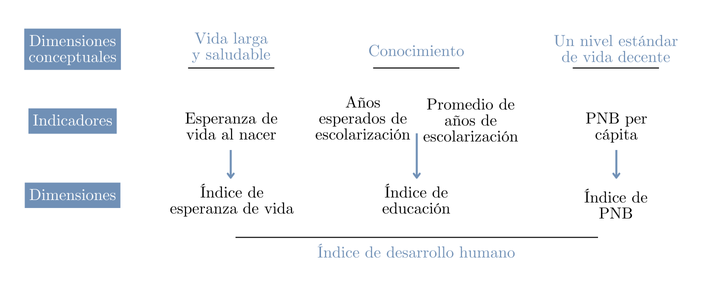
\includegraphics{diagrama1.png}

\[IDH = \Bigl(\text{Índice de esperanza de vida}\times\text{Índice de educación}\times\text{Índice de ingreso}\Bigl)^{1/3}\]

Todos estos índices de dimensión se calculan de la siguiente forma:

\[\text{Índice de dimensión}=\frac{\text{valor actual - valor mínimo}}{\text{valor máximo - valor mínimo}}\]

Los valores mínimo y máximo están definidos para transformar la variable
en un indicador con valores entre 0 y 1 y se llaman ``cero natural'' y
``objetivo aspiracional'', respectivamente.

\hypertarget{vida-larga-y-saludable}{%
\subsubsection{Vida larga y saludable}\label{vida-larga-y-saludable}}

La primer componente del IDH es vida larga y saludable, que sin dudas
promueve el desarrollo humano y es primordial para mantener un buen
estilo de vida. Actualmente, el indicador que representa este aspecto se
obtiene a partir de la esperanza de vida al nacer. Entendiendo a la
esperanza de vida al nacer como número medio de años que un recién
nacido podría esperar vivir, si transcurriera su vida expuesto a las
tasas de mortalidad específicas por sexo y edad vigentes en el momento
de su nacimiento, para un año concreto, en un país, territorio o zona
geográfica determinados.

Para el cálculo del IDH se transforma la esperanza de vida al nacer en
un índice calculado con el índice de dimensión mencionado anteriormente.
Para esto se definen valores mínimos y máximos de la esperaza de vida.
La elección del cero natural para la esperanza de vida es de 20 años y
está basada en evidencia histórica que muestra que ningún país en el
siglo 20 ha tenido una esperanza de vida menor a los 20 años. El valor
máximo u objetivo aspiracional está definido a los 85 años ya que es un
objetivo realista al que muchos países pueden aspirar, especialmente por
las constantes mejoras en las condiciones de vida y los avances médicos.

De esta forma el índice de esperanza de vida se calcula de la siguiente
forma:

\[\text{Índice de esperanza de vida} = \frac{\text{Esperanza de vida al nacer}-20}{85-20}\]

\hypertarget{conocimiento}{%
\subsection{Conocimiento}\label{conocimiento}}

En representación de la dimensión ``Conocimiento'', se incluye al
cálculo del IDH el índice de educación. Este se calcula como una media
aritmética entre dos indicadores de dimensión para las variables años
esperados de escolaridad y años promedio de escolaridad.

Los años esperados de escolaridad refieren al número de años de
escolaridad que puede esperar recibir un niño en edad de comenzar la
escuela, si los patrones vigentes de las tasas de matriculación por edad
se mantienen a lo largo de su vida. Y los años medios de escolaridad son
el número promedio de años de educación recibidos por las personas de 25
años o más, calculado a partir de los niveles de logros educativos
utilizando la duración oficial de cada nivel.

Resulta necesario aclarar que para la rama del conocimiento, al tomarse
dos indicadores en vez de uno, primero se calcula el índice de dimensión
de ambos y, a continuación, se obtiene la media aritmética de los dos
índices resultantes.

\[\text{Índice de años esperados} = \frac{\text{Años esperados de escolaridad}-0}{18-0}\]

\[\text{Índice de años medios} = \frac{\text{Años medios de escolaridad}-0}{15-0}\]

Las sociedades pueden subsistir sin educación formal, lo que justifica
la educación mínima de 0 años. El máximo de años esperados de
escolaridad, 18, equivale a la obtención de un máster en la mayoría de
los países. El máximo de años medios de escolaridad, 15, es el máximo
previsto de este indicador para 2025.

El índice de educación queda definido entonces como la media aritmética
de los índices mencionados:

\[\text{Índice de educación} = \frac{\text{Índice años esperados de escolaridad}+\text{Índice años medios de escolaridad}}{2}\]

\hypertarget{nivel-estuxe1ndar-de-vida-decente}{%
\subsection{Nivel estándar de vida
decente}\label{nivel-estuxe1ndar-de-vida-decente}}

Se considera que un nivel estándar de vida se puede alcanzar cuando la
nación en la que se reside tiene un alto producto bruto interno per
cápita, que refiere al valor monetario de la producción de bienes y
servicios de demanda final de un país o región durante un período
determinado para cada habitante de la población. Es por eso que el PBI
fue la variable considerada en el cálculo del IDH en un principio.

Sin embargo, a partir del año 2010, para medir el nivel de vida, el
producto nacional bruto (PNB) per cápita reemplaza al producto interno
bruto (PIB) per cápita. Esto se debe a que en un mundo globalizado,
suele haber grandes diferencias entre los ingresos de los residentes de
un país y su producto interno. Parte de lo que ganan los habitantes se
envía al extranjero, algunas personas reciben remesas del exterior y
algunos países reciben considerables flujos de ayuda.

Se define al producto nacional bruto (PNB) per cápita como los ingresos
totales de una economía generados por su producción y la propiedad de
los factores de producción, menos los ingresos pagados por el uso de
factores de producción que son propiedad del resto del mundo,
convertidos a dólares internacionales usando las tasas de la PPA, y
divididos por la población a mitad del año.

Para comparar el estándar de vida entre los países, los datos deben
ajustarse por la paridad del poder adquisitivo (PPA) a fin de eliminar
las diferencias en el valor de un dólar entre países. Se entiende por
paridad de poder adquisitivo (PPA) al tipo de cambio que refleja las
diferencias de precios entre países y permite hacer comparaciones
internacionales del producto e ingreso reales. En la tasa de PPA en US\$
(utilizada en este Informe), US\$1 en PPA tiene el mismo poder
adquisitivo en la economía de cualquier país que US\$1 en los Estados
Unidos de América.

En el \emph{IDH} se calcula el índice de ingreso como

\[\text{Índice de ingreso} = \frac{PNB - 100}{75.000-100}\]

El bajo valor mínimo para el Producto Nacional Bruto per cápita se
considera en los 100 dólares, el uso de este valor se justifica por la
considerable cantidad de producción de subsistencia y producción no
comercial no medida en economías cercanas al mínimo, que no se captura
en los datos oficiales. Por otro lado, el valor máximo se establece en
75.000 dólares per cápita. Kahneman y Deaton (2010) han demostrado que
prácticamente no hay ganancia en desarrollo humano y bienestar con un
ingreso anual per cápita superior a 75,000 dólares. Actualmente solo
cuatro países (Brunei Darussalam, Liechtenstein, Qatar y Singapur)
superan el techo de ingresos per cápita de 75,000 dólares.

DESDE ACÁ REVISAR \emph{Lo que sigue está sacado de lo de 2022}

La base de datos de Indicadores del Desarrollo Mundial del Banco Mundial
de 2022 contiene estimaciones del GNI per cápita en términos de paridad
de poder adquisitivo (PPP) constantes de 2017 para muchos países. Para
los países que no tienen este indicador (total o parcialmente), la
Oficina del Informe sobre Desarrollo Humano (HDRO) lo calcula
convirtiendo el GNI per cápita en moneda local de términos corrientes a
términos constantes usando dos pasos. Primero, el valor del GNI per
cápita en términos corrientes se convierte en términos PPP para el año
base (2017). Segundo, se construye una serie temporal del GNI per cápita
en términos constantes de PPP de 2017 aplicando las tasas de crecimiento
real al GNI per cápita en términos de PPP para el año base. La tasa de
crecimiento real se implica por la proporción del crecimiento nominal
del GNI per cápita en moneda local corriente al deflactor del PIB.

Para varios países sin un valor de GNI per cápita en términos constantes
de PPP de 2017 para 2021 reportado en la base de datos de Indicadores
del Desarrollo Mundial, se aplican tasas de crecimiento real del PIB per
cápita disponibles en la base de datos de Indicadores del Desarrollo
Mundial o en la base de datos Perspectivas de la Economía Mundial del
Fondo Monetario Internacional a los valores más recientes de GNI en
términos constantes de PPP. Las tasas de conversión oficiales de PPP son
producidas por el Programa de Comparación Internacional, cuyas encuestas
recolectan periódicamente miles de precios de bienes y servicios
comparables en muchos países. La última ronda de este ejercicio se
refiere a 2017 y cubrió 176 economías.

Las tasas de conversión oficiales de PPP son producidas por el Programa
de Comparación Internacional, cuyas encuestas recolectan periódicamente
miles de precios de bienes y servicios comparables en muchos países.

----- Durante la investigación se debate cada una de estas dimensiones
que componen el IDH con la finalidad de cuestionarlos e intentar una
reformulación que sea más realista para los tiempos que corren.

\pagebreak

\hypertarget{cuestionamiento}{%
\section{Cuestionamiento}\label{cuestionamiento}}

Si bien se piensa que el calculo del IDH actual logra reflejar muchas
cuestiones vinculadas a lo que hace que un país se pueda considerar con
mayor o menor desarrollo humano, hay otros aspectos de lo que se define
como desarrollo humano que no son tenidos en cuenta.

En primer lugar, se menciona que no se toma por sentado que el
crecimiento económico conduce a un mayor bienestar para todos sino que
los ingresos se considera un medio para el desarrollo, más que un fin en
sí mismo. Esto indica que si bien una medida como el Producto Nacional
Bruto podría ser un medio para explicar si un país esta más o menos
desarrollado no podría definir esto por completo, ya que el tener un
valor alto de \emph{PBI} no garantizaría el bienestar de toda la
población. A partir de esta problemática surge la idea de implementar
otra variable de corrección en esta dimensión para así poder tener en
cuenta otras cuestiones del desarrollo humano para el nivel de vida de
las personas.

Poniendo el foco en la dimensión de una vida larga y saludable, se puede
identificar que en un principio el mismo nombre de esta dimensión no
esta completamente explicado por la variable que se utiliza ya que la
esperanza de vida solo indicaría si las personas tienen una vida larga o
corta, pero no se determina qué tan saludable es. Por esta razón, en
esta dimensión se considera importante incorporar otra variable que
pueda tener en cuenta las condiciones en las que se viven, en cuanto a
salud, en los distintos países.

Por otro lado, la definición de desarrollo humano menciona que este
consiste en ofrecer oportunidades a las personas, no de insistir en que
las aprovechen. Es decir, que las personas tengan la libertad de llevar
a cabo la vida que ellos elijan sin imponerles cómo vivirla. Esto no se
tiene en cuenta actualmente en el indice ya que no se calcula una
dimensión de libertad. Se considera que podría ser una propuesta
adecuada incluir una cuarta dimensión al indice de desarrollo humano que
tenga en cuenta cuestiones relacionadas con la libertad de las personas
en su día a día.

\hypertarget{propuestas-y-modificaciones}{%
\section{Propuestas y
modificaciones}\label{propuestas-y-modificaciones}}

En esta sección se explica cada una de las modificaciones propuestas
para este nuevo índice, acompañado del razonamiento realizado. Además,
se muestran otras posibles propuestas que se podrían llevar a cabo en
investigaciones futuras o descartadas del presente desarrollo por
diversas razones.

\hypertarget{vida-larga-y-saludable-1}{%
\subsection{Vida larga y saludable}\label{vida-larga-y-saludable-1}}

\hypertarget{debate}{%
\subsubsection{Debate}\label{debate}}

Como se mencionó anteriormente, tener una alta esperanza de vida sin
dudas logra una vida larga, pero no necesariamente saludable. Esta
variable no proporciona información sobre la calidad de vida en el
horizonte de años de vida y si este horizonte se desarrolla con buena
salud o, por el contrario, se desarrolla con alguna discapacidad o
dependencia. Es por esto que se propone hacer uso de la
\textbf{Esperanza de vida en buena salud al nacer} para cuantificar este
aspecto según la cantidad de años de calidad y no sólo en cantidad de
años.

Se considera condición de buena salud a la ausencia de limitaciones
funcionales o de discapacidad ya que las enfermedades crónicas, los
problemas mentales y la discapacidad física aumentan su prevalencia con
la edad y reducen la calidad de vida de las personas que sufren estas
condiciones de salud. La esperanza de vida en buena salud al nacer es
una medida que combina información de mortalidad y de morbilidad y se
calcula, según el Instituto de Estadística español, en base al método
Sullivan ( a traves de tablas de mortalidad) y al indicador de
limitaciones generales de actividad de Euro-REVES (Network on Health
Expectancy).

El método de Sullivan es un método estadístico que combina la
información de las tablas de mortalidad con datos sobre la prevalencia
de morbilidades o limitaciones en la actividad. Ajustando las tablas de
mortalidad con la prevalencia de morbilidad, se calcula la esperanza de
vida libre de limitaciones, sumando los años de vida ajustados para
obtener una medida integral de salud poblacional. Este método
proporciona una visión clara de los años que se espera que una persona
viva en buena salud, combinando la cantidad y calidad de vida.

En resumen, la organización mundial de la salud define al calculo de la
esperanza de vida en buena salud al nacer de la siguiente manera:

\[HALE_x = \Biggl[\sum_{i=x}^w YWD_i\Biggl] \Bigl/ I_x\]

donde:

\begin{itemize}
\item
  \(YWD_x = L_x (1-D_x)\) son los años vividos sin discapacidad entre la
  edad \(x\) y \(x+5\)
\item
  \(I_x\) es el número de sobrevivientes a las edad \(x\)
\item
  \(L_x\) es el total de años vividos entre la edad \(x\) y \(x+5\) de
  la tabla de vida
\item
  \(D_x\) es la proporción de gente con discapacidad entre los años
  \(x\) y \(x+5\)
\end{itemize}

También se investigaron medidas alternativas sobre la capacidad de
disfrutar de una vida saludable, pero no se ha encontrado ninguna opción
mejor o más viable que la esperanza de vida al nacer.

\hypertarget{modificaciuxf3n-en-el-cuxe1lculo-del-idh}{%
\subsubsection{Modificación en el cálculo del
IDH}\label{modificaciuxf3n-en-el-cuxe1lculo-del-idh}}

La esperanza de vida en buena salud al nacer es una variable que
contiene más información e identifica mejor a la dimensión ``tener una
vida larga y saludable''. Ahora bien, ¿cómo incluirla al cálculo de IDH?
Se han barajado algunas opciones:

\textbf{completar segun descriptivo}

\begin{itemize}
\item
  Reemplazar la esperanza de vida al nacer por la esperanza de vida en
  buena salud al nacer directamente en el cálculo del índice de salud.
  Algunas cuestiones que limitaron esta decisión fue el hecho de que no
  todos los países tienen esta medida, mientras que la esperanza de vida
  al nacer es más común y accesible. De esta forma, se estaría
  subestimando el valor del IDH para aquellos países que no tienen la
  posibilidad de aportar un índice de salud, aún así teniendo un
  resultado alto en la esperanza de vida al nacer.
\item
  Tomar ambas variables y promediarlas previo al cálculo del índice.
  Esta opción fue rápidamente descartada por el hecho de que ambas
  variables resumen aspectos muy similares, están muy relacionadas.
\item
  Penalizar la esperanza de vida al nacer, disminuyendo su valor en
  aquellos países donde la esperanza de vida en buena salud al nacer es
  notablemente menor. La determinación de la penalización propuesta y la
  elección de valores mínimo y máximo involucraría pensamientos
  subjetivos. Esta opción se lleva a cabo tranformando los dos valores
  en indicadores y despues multipliacandolos, de este forma el valor
  anteriormente obtenido para el índice de salud baja apenas en aquellos
  paises con esperanza de vida saludable mucho menor a la esperanza de
  vida.
\item
  Se podría pensar incoporar tambien la diferencia entre esperanza de
  vida al nacer y la espereranza de vida saludable al nacer de alguna
  manera. Sin embargo, esta idea es más subjetiva ya que valores grandes
  de esta diferencia se pueden considerar como positivos o negativos
  dependiendo de que lado se vea. Si bien primarimente se pensó que una
  gran diferencia significaba un país con menor desarrollo ya que
  simbolizaba que muchos de los años vividos eran en mala salud, luego
  se pensó que también esta gran diferencia podía simbolizar que el país
  en cuestión contaba con una gran tecnología y una avanzada medicina
  que hacía que los pacientes vivan más años a pesar de sus condiciones
  de salud. Si el desarrollo se plantea por el lado de avances en la
  humanidad entonces si la diferencia es grande se podría considerar
  como un mayor índice de desarrollo, por lo dicho anteriormente.
\end{itemize}

\hypertarget{conocimiento-1}{%
\subsection{Conocimiento}\label{conocimiento-1}}

JUSTIFICCACIÓN DE NO CAMBIO CONOC

\emph{Falta explicar cómo era antes de la modificación porque estamos de
acuerdo} Antes del año 2010, se tenían en cuenta las variables
alfabetización y matriculación bruta en la dimensión de conocimientos.

En el ámbito de los conocimientos, los años promedio de instrucción
sustituyen a la alfabetización y la matriculación bruta se replanteó
como los años esperados de instrucción, es decir, los años de educación
que un niño puede esperar recibir dada la tasa de matriculación vigente.
Cada vez más países calculan con mayor frecuencia los años promedio de
instrucción. Dicha medida permite distinguir mejor entre países,
mientras que los años esperados de instrucción son consistentes con la
reformulación de esta dimensión en términos de años.

Lo ideal sería que las mediciones de la dimensión de conocimientos
incorporasen evaluaciones de calidad, tal como se ha hecho en varios
informes sobre desarrollo humano nacionales y regionales. Por ejemplo,
el Informe de los Estados Árabes de 2003 creó una medida tanto de la
cantidad como de la calidad de la educación. Ésta ajusta los años
promedio de instrucción con puntajes promedio en pruebas e incluye
indicadores vinculados con medios de difusión, comunicaciones y
científicos capacitados. Pero no existen buenas medidas sobre la calidad
de la educación para una cantidad suficiente de países; las evaluaciones
internacionales sobre conocimientos científicos y matemáticos y
habilidades de lecto-escritura de los jóvenes son instrumentos de gran
valor, pero su cobertura es baja y su frecuencia, irregular.

Es por lo dicho anteriormente, que se decide dejar esta dimensión sin
modificaciones pero con una propuesta futura de encontrar algún tipo de
medición que pueda reflejar la calidad de la educación en los distintos
paises.

\hypertarget{nivel-estuxe1ndar-de-vida-decente-1}{%
\subsection{Nivel estándar de vida
decente}\label{nivel-estuxe1ndar-de-vida-decente-1}}

\hypertarget{debate-1}{%
\subsubsection{Debate}\label{debate-1}}

Una de las principales preocupaciones al analizar el cálculo del índice
de desarrollo humano actual fue la falta de consideración de uno de los
primeros aspectos que se mencionan en la definición de desarrollo humano
el cual establece que no se toma por sentado que el crecimiento
económico conduce a un mayor bienestar para todos. Al utilizar el
\emph{PNB} para medir la dimensión de nivel estándar de vida decente se
esta tomando en cuenta solamente el desarrollo económico de un país para
explicar que tan bueno es el nivel de vida de este.

Se piensa que en ciertas situaciones puede haber un país con un gran
valor de PNB pero en donde las riquezas no estén distribuidas
equitativamente. Es decir, quizás este valor de PNB es alto por un bajo
porcentaje de la población quien lo acumula mientras que existe un gran
porcentaje de personas que no viven un nivel de vida decente. Es por
esta razón que se considera incorporar en esta dimensión el indice de
Gini.

El coeficiente Gini es el método más utilizado para medir la desigualdad
salarial. Es una herramienta analítica que suele emplearse para medir la
concentración de ingresos entre los habitantes de una región, en un
periodo de tiempo determinado. Fue desarrollada por el estadístico
italiano Corrado Gini en 1912, representando con 0 a una igualdad
perfecta y con un 100 a una desigualdad perfecta.

Este indicador se calcula como el área entre la curva de Lorenz y una
línea hipotética que representa la igualdad total. Esta gráfica se
utiliza a través de dos ejes de coordenadas, para identificar de forma
sencilla el porcentaje de ingresos que corresponde a un porcentaje de
población.

\begin{figure}

{\centering \includegraphics{Informe_files/figure-latex/unnamed-chunk-1-1} 

}

\caption{Índice de Gini en un caso hipotético}\label{fig:unnamed-chunk-1}
\end{figure}

Para comprender la lógica, se puede observar en la Figura 1 que el 50\%
alcanza un 25\% del ingreso mientras que un 75\% de la población llega a
más del 50\% del ingreso, es decir, el ingreso que logra el 50\% de la
población lo alcanza el 20\% contiguo, lo cual indica desigualdad ya que
el ingreso no estaría equitativamente distribuído.

Se propone incorporar el índice de Gini al cálculo del IDH como (1-GINI)
para que un país más desigual en términos salariales tenga menos
desarrollo.

\hypertarget{modificaciuxf3n-en-el-cuxe1lculo-del-idh-1}{%
\subsubsection{Modificación en el cálculo del
IDH}\label{modificaciuxf3n-en-el-cuxe1lculo-del-idh-1}}

\textbf{completar} -------------------------------

\hypertarget{modificaciuxf3n}{%
\subsubsection{Modificación}\label{modificaciuxf3n}}

\textbf{explicar diferentes formas de meter indice de gini a esta
dimension y cual se elige y porque}

\hypertarget{rama-nueva}{%
\subsection{RAMA NUEVA}\label{rama-nueva}}

Cosas para justificar la rama nueva

\hypertarget{debate-2}{%
\subsection{Debate}\label{debate-2}}

\emph{Informe IDH 2010} El nuevo IDH poseía algunas debilidades, como lo
reconocieron los autores; entre ellas, la dependencia de los promedios
nacionales ---que ocultaban sesgos de distribución--- y la falta de una
``medida cuantitativa de la libertad humana''. No obstante, logró
plantear sin problemas la tesis central del Informe, declarada
brevemente ya en la primera frase: ``La verdadera riqueza de una nación
está en su gente''. Veinte años después, la brillantez conceptual y la
importancia del paradigma original del desarrollo humano siguen siendo
indiscutibles. Existe un consenso casi universal sobre la imposibilidad
de medir el éxito de un país o el bienestar de un individuo únicamente a
partir de su ingreso. Si bien el ingreso es fundamental, ya que sin
recursos cualquier avance es difícil de lograr, también debemos tomar en
cuenta si la gente puede llevar una vida saludable y prolongada, si
tiene oportunidad de recibir educación y si es libre de aplicar sus
conocimientos y talentos para configurar su propio destino. Hacia el
futuro, los próximos informes deberán lidiar con temas aún más
complejos, entre ellos el ámbito cada vez más crítico de la
sostenibilidad, la desigualdad y nociones más amplias de empoderamiento.
Mientras eso sucede, los nuevos desafíos que enfrentamos son aún más
graves, como aquellos relacionados con la conservación del medio
ambiente y la sostenibilidad de nuestro bienestar y de las libertades
básicas.

Durante los últimos 20 años, el IDH ha sido objeto de críticas. Algunas
se relacionan con su construcción y composición, mientras otras sugieren
que debería ampliarse e incluir más dimensiones, desde igualdad de
género hasta biodiversidad. Muchas de las inquietudes son válidas. Pero,
el objetivo no es crear un indicador incuestionable del bienestar, sino
reorientar la atención hacia un desarrollo enfocado en el ser humano y
alimentar el debate sobre cómo propiciar el progreso de las sociedades.
Mientras más discutimos sobre qué debe incluirse o no en el IDH ---ya
sea si tiene sentido agrupar distintas categorías, cuánta importancia
darle a cada una o cómo conseguir más y mejores datos--- más se aleja el
debate del estrecho enfoque en el crecimiento que dominó la reflexión
sobre el desarrollo. El IDH ha resultado tremendamente fructífero como
alternativa al enfoque basado solamente en el ingreso.

\emph{VER A PARTIR DE LA PAG 29 DE INFORME 2020} \#\#\# Modificación IDH

\hypertarget{cuxe1lculo-de-idh-modif}{%
\section{Cálculo de IDH modif}\label{cuxe1lculo-de-idh-modif}}

Antes o como secciones de esta explicar de dónde sacamos los datos, qué
hicimos con los datos faltantes.

\hypertarget{estimaciuxf3n-de-datos-faltantes}{%
\subsection{Estimación de datos
faltantes}\label{estimaciuxf3n-de-datos-faltantes}}

For a small number of countries missing one of the four indicators, the
HDRO estimated the missing values using crosscountry regression models.
In this Report expected years of schooling were estimated for Bahamas,
Dominica, Equatorial Guinea, Haiti, Libya, Papua New Guinea, Tonga,
Trinidad and Tobago, and Vanuatu. Mean years of schooling were estimated
for Eritrea, Grenada and Saint Kitts and Nevis.

\hypertarget{resultados}{%
\section{Resultados}\label{resultados}}

\begin{itemize}
\item
  Rankear los países con IDH modificado y comparar (2 graficos países
  colores)
\item
  Corr entre los IDH y el/los modificados
\item
  Resulta diferente o no al IDH ventajas y desventajas
\item
  Idea mirando las tablas del informe del idh compara la clasificación
  de IDH con IDH modif por desigualdad viendo la diferencia. Ver si se
  podría y valdría la pena hacer lo mismo con el nuestro
\end{itemize}

\hypertarget{cosas-que-quedan-propuestas}{%
\section{Cosas que quedan
propuestas}\label{cosas-que-quedan-propuestas}}

\hypertarget{conclusiuxf3n}{%
\section{Conclusión}\label{conclusiuxf3n}}

\hypertarget{categoruxedas-seguxfan-desarrollo-humano}{%
\section{Categorías según desarrollo
humano}\label{categoruxedas-seguxfan-desarrollo-humano}}

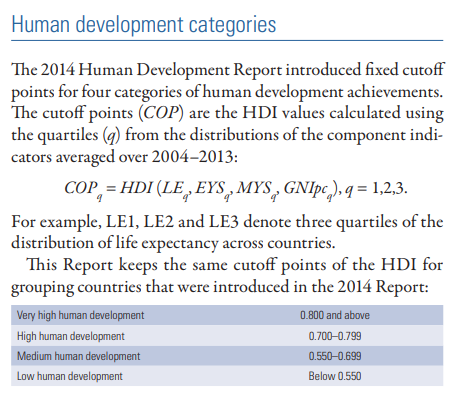
\includegraphics{agregar1.png}

Aggregate HDI values for country groups (by human development category,
region and the like) are calculated by applying the HDI formula to the
weighted group averages of component indicators. Life expectancy and GNI
per capita are weighted by total population, expected years of schooling
is weighted by population ages 5--24 and mean years of schooling is
weighted by population ages 25 and older.

\pagebreak

\hypertarget{guuxeda-de-cosas-que-tienen-que-estar}{%
\section{GUÍA DE COSAS QUE TIENEN QUE
ESTAR}\label{guuxeda-de-cosas-que-tienen-que-estar}}

\begin{itemize}
\item
  \emph{Antes de nombrar la modificación que proponemos deberíamos
  nombrar algo de críticas al IDH y otras modificaciones que ya se
  hicieron (Informe ver en Documentos) y por qué buscamos una distinta
  que queremos mostrar.} EN 2010, se incorporan tres nuevos indicadores
  que capturan la desigualdad multidimensional, las disparidades de
  género y las privaciones extremas. El Índice de Desarrollo Humano
  ajustado por la Desigualdad, el Índice de Desigualdad de Género, así
  como el Índice de Pobreza Multidimensional \emph{CAP 5 P106 DEL
  INFORME 2010}
\item
  Orden posible:

  \begin{itemize}
  \tightlist
  \item
    \emph{Intro + objetivo: definicion del desarrollo humano segun idh y
    segun nosotros}
  \item
    terminos
  \item
    Definición del calculo IDH actual y calculo de cada dimensión y
    explicación
  \item
    Críticas / Otas modificaciones que ya se hicieron + Por qué
    proponemos igual hacer uno nuevo
    \url{https://www.undp.org/sites/g/files/zskgke326/files/2023-09/notas_tecnicas.pdf}
  \item
    Explicación de modificaciones en cada dimensión (incluyendo
    posibilidades que se nos ocurrieron pero no hicimos o que
    descartamos o que estarían bueno hacer). Explicar tmb la de Derechos
    y libertades.
  \item
    Cálculo final IDH modif (1 o los que sean) Aclarar acá o arriba de
    donde se obtuvieron los datos
  \item
    Resultados (ver abajo opciones)
  \item
    Conclusiones
  \item
    En algún lado un apartado con cosas que quedan propuestas si es
    necesario.
  \item
    Bibliografía
  \end{itemize}
\item
  Acordarnos de explicar para las variables que lo hayamos hecho que
  tomamos valores 2019 o más cercano
\end{itemize}

\hypertarget{eleccion}{%
\subsection{eleccion}\label{eleccion}}

Elección: el desarrollo humano consiste, fundamentalmente, en una mayor
capacidad de elección. Se trata de ofrecer oportunidades a las personas,
no de insistir en que las aprovechen. Nadie puede garantizar la
felicidad humana, y las decisiones que tomen las personas son asunto
suyo. El proceso de desarrollo -desarrollo humano- debería al menos
crear un entorno para que las personas, individual y colectivamente,
desarrollen todo su potencial y tengan una oportunidad razonable de
llevar una vida productiva y creativa que valoren.

\#Bibliografia

De donde sacamos los datos y lugares con info, informe idh\ldots{}

\end{document}
